
\begin{frame}[noframenumbering,plain]
    \vfill
    \mytitle{Introduction}
    \bigskip
    \begin{center}
        \only<-1>{\textbf{\bgreen{Sketch-based} \textcolor{gray}{approaches to} \borange{process} \bred{massive} \bblue{string data}}}
        \pause
        \only<2>{\textbf{\textcolor{gray}{Sketch-based approaches to process massive} \bblue{string data}}}
    \end{center}
    \vfill
\end{frame}

\def\stringseashells{S,h,e,\_,s,e,l,l,s,\_,s,e,a,s,h,e,l,l,s,\_,b,y,\_,t,h,e,\_,s,e,a,s,h,o,r,e}
\def\stringstruggled{I, ,s,t,r,u,g,g,l,e,d, ,t,o, ,m,a,k,e, ,t,h,i,s, ,f,i,g,u,r,e, ,w,i,t,h, ,t,i,k,z,!}


\begin{frame}{Strings}
    A string $T$ of length $n$ is a sequence $T[0]T[1]...T[n-1]$ of characters from a finite alphabet $\Sigma$ of size $\sigma$.\\
    \begin{center}
        \begin{tikzpicture}[x = 2em]
            \node (t) at (-0.8,0) {\smash{$T=$}$\vphantom{m}$};
            \numberedstring{\stringstruggled};
            \only<2|handout:0>{
                \numberedsubstring[blue]{\stringstruggled}{8}{18};
                \node at (13*0.25,-0.5) {$T[8..18]$};
            }
            \only<3>{
                \numberedsubstring[blue]{\stringstruggled}{0}{9};
                \node at (5*0.25,-0.5) {$T[0..9]$ is a prefix};
            }
            \only<4>{
                \numberedsubstring[blue]{\stringstruggled}{25}{42};
                \node at (33*0.25,-0.5) {$T[25..41]$ is a suffix};
            }
        \end{tikzpicture}
        \\
    \end{center}
    \textbf{Definitions and Notations}\\
    The \textbf{substring} from position $i$ to position $j$: $T[i]T[i+1]...T[j]$ is denoted $T[i..j]$.\\
    Substrings of the form $T[0..j]$ are \textbf{prefixes}.\\
    Substring of the form $T[i..n-1]$ are \textbf{suffixes}.
    \pause \pause
\end{frame}

\begin{frame}{Strings}
    Simple and versatile, any file can be seen as a string.
    They are used in fields such as \bgreen{Bioinformatics}, \bblue{Information Retrieval}, and \borange{Cyber-security}.

    \medskip
    \begin{tabular}{l  c c c c}
        \emph{Strings} & Binary file & DNA sequence & ASCII text file & UTF-8 text file \\
        \rule{0pt}{10ex}    
        &
        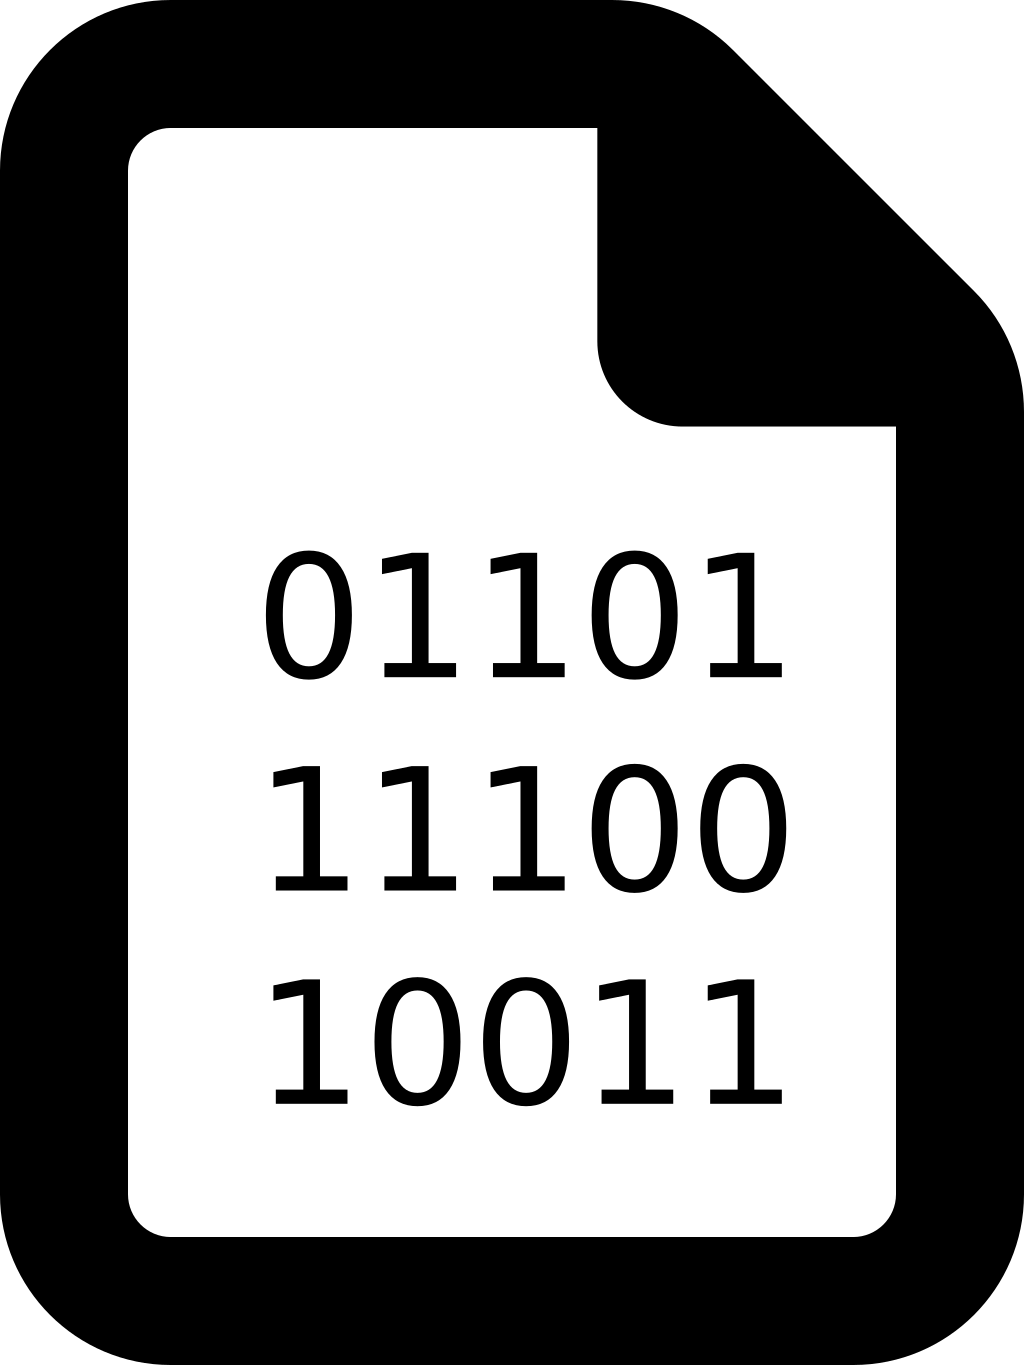
\includegraphics[width=1cm]{pictures/file-bin.png}&
        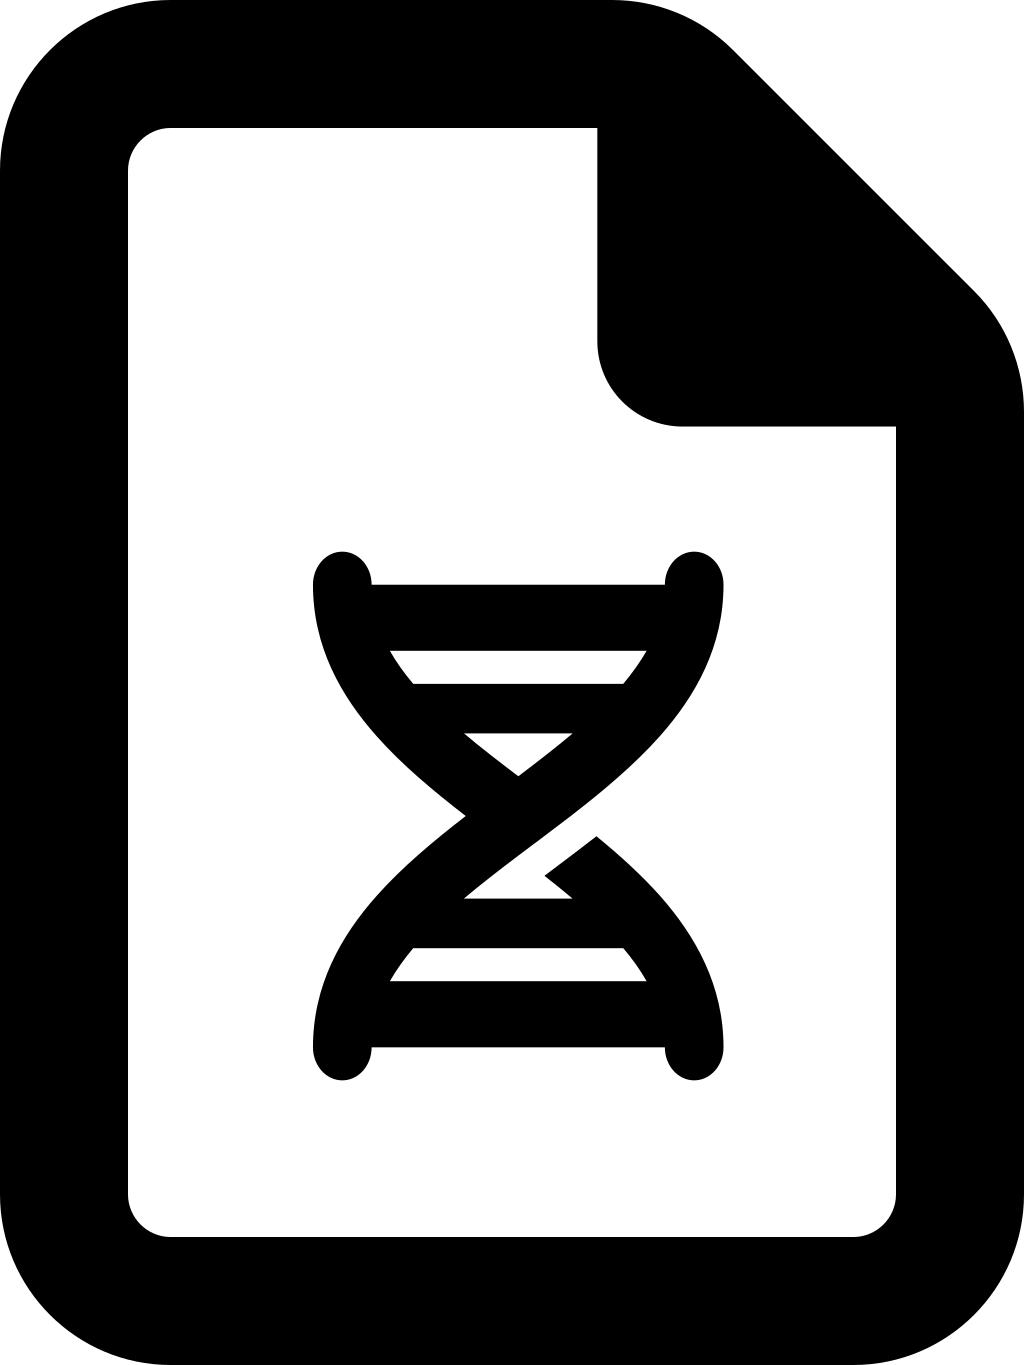
\includegraphics[width=1cm]{pictures/file-dna.png}&
        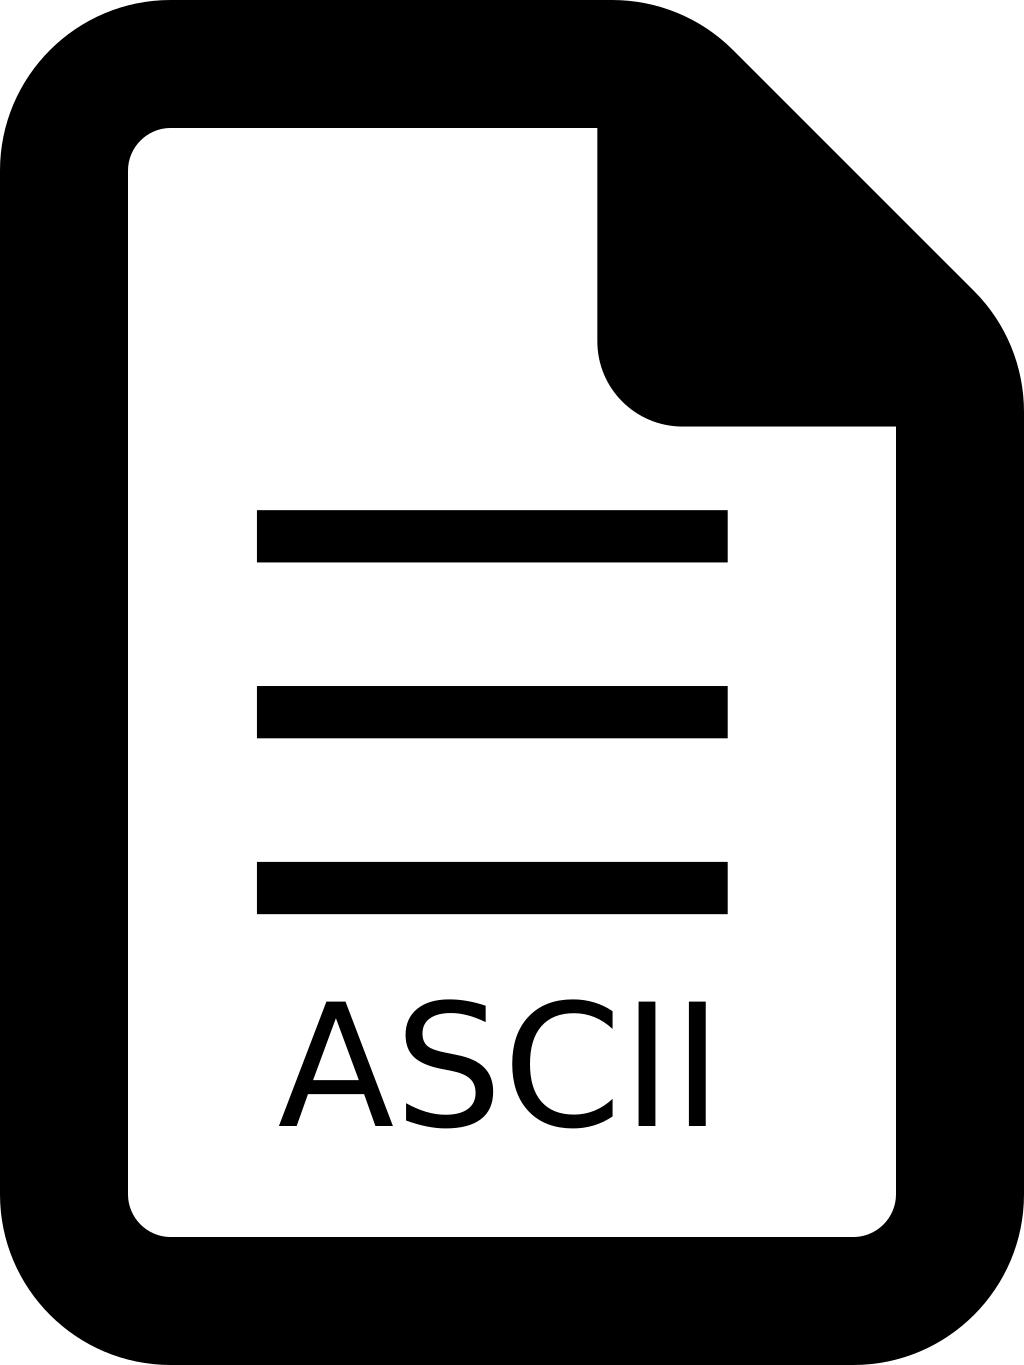
\includegraphics[width=1cm]{pictures/file-ascii.png}&
        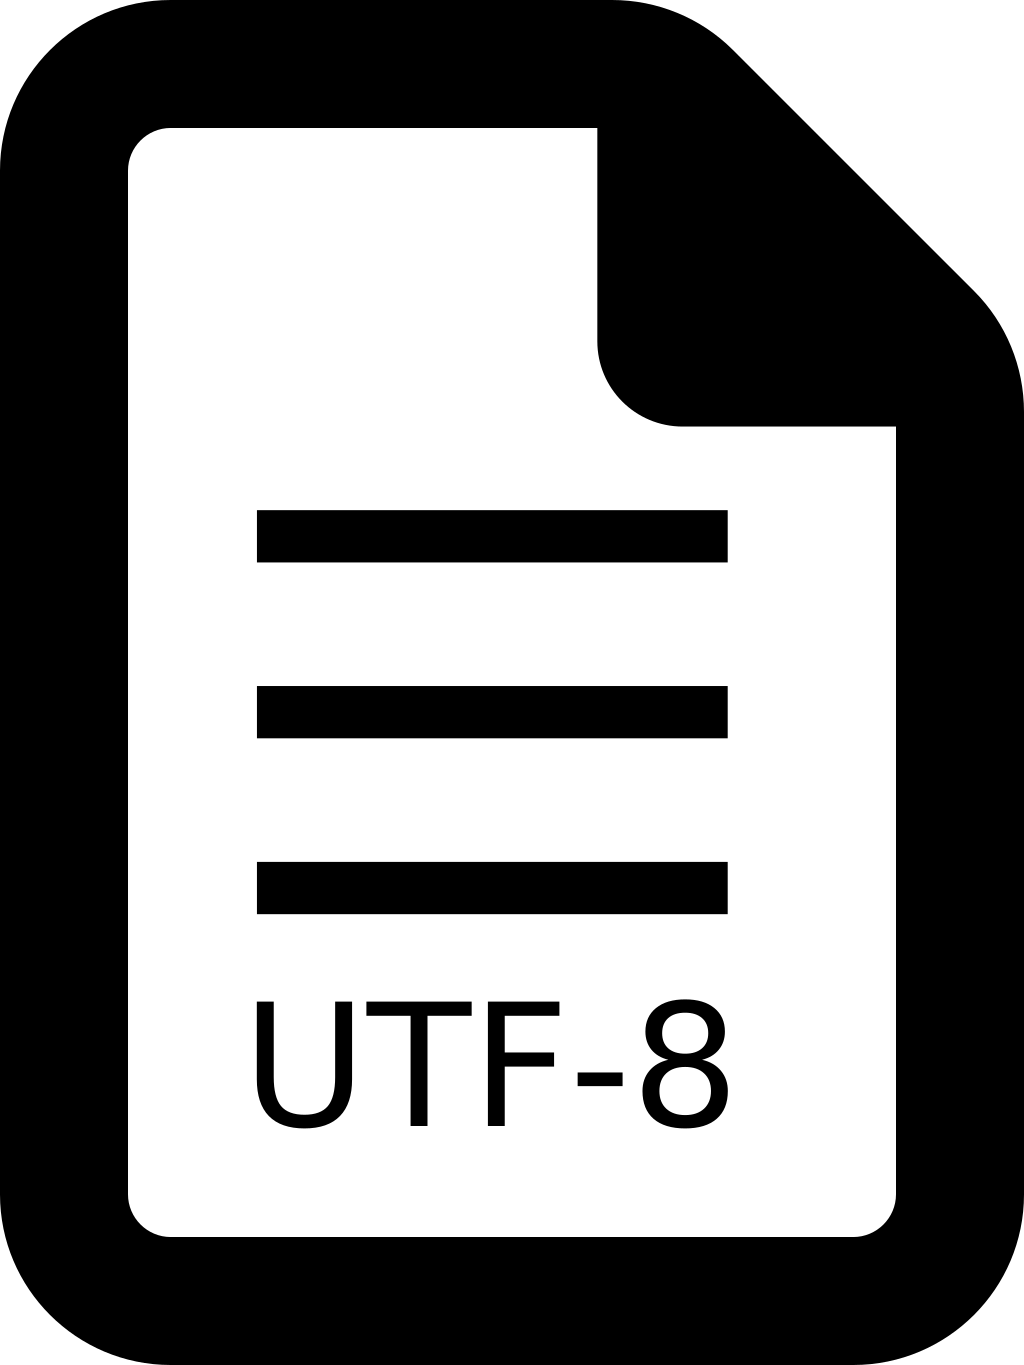
\includegraphics[width=1cm]{pictures/file-utf-8.png}
        \\
        \rule{0pt}{4ex}  
        \emph{Alphabets} & $\Sigma=\{0,1\}$ & $\Sigma=\{\texttt{A,T,C, G}\}$ & $\sigma=128$ & $\sigma = 1,112,064$\\
    \end{tabular}
    \medskip

    Most natural task: Given a pattern $P =$ \texttt{th}, does it occur in  $T$ and where ?

    \begin{center}
        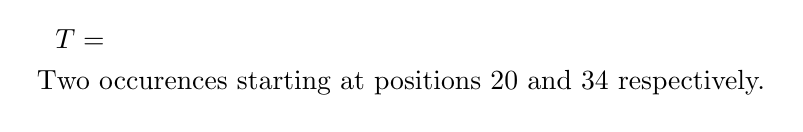
\begin{tikzpicture}[x = 2em]
            \node (t) at (-0.8,0) {\smash{$T=$}$\vphantom{m}$};
            \numberedstring{\stringstruggled};
            \numberedsubstring[myorange]{\stringstruggled}{20}{21};
            \numberedsubstring[myblue]{\stringstruggled}{34}{35};
            \only<1>{
                \node at (20*0.25,-0.5) {
                    Two occurences starting at positions \borange{20} and \bblue{34} respectively.
                };
            }
        \end{tikzpicture}
        \\
    \end{center}

\end{frame}


\begin{frame}{Classic Pattern Matching}

\end{frame}

\begin{frame}{Algorithms vs Data-structures}

\end{frame}

\begin{frame}{Classic Indexing the suffix tree}

\end{frame}

\begin{frame}[noframenumbering,plain]
    \vfill
    \mytitle{Introduction}
    \bigskip
    \begin{center}
        \textbf{\textcolor{gray}{Sketch-based approaches to \borange{process} \bred{massive} string data}}
    \end{center}
    \vfill
\end{frame}

\begin{frame}{Challenges: Processing tasks}
3 categories of task (for this thesis)
Complex Matching
Repetition detection
Similarity Measures and distances
\end{frame}

 \begin{frame}{Complex Matching}
    
 \end{frame}

 \begin{frame}{Repetition detection}
    
 \end{frame}

 \begin{frame}{Similarity Measures and distances}
    
 \end{frame}

\begin{frame}{Challenges: the scale}
    A visualization as done for the loreal poster (starting a the base of wikipedia, which seems already very large)
    And still growing
\end{frame}

\begin{frame}{Challenges: the scale}
    The largest archive are only searchable by metadata (and already it requires significant efforts...)
    And the 
\end{frame}

\begin{frame}[noframenumbering,plain]
    \vfill
    \mytitle{Introduction}
    \bigskip
    \begin{center}
        \textbf{\textcolor{gray}{\bgreen{Sketch-based} approaches to process massive string data}}
    \end{center}
    \vfill
\end{frame}

\begin{frame}{What is a sketch ?}
    \begin{columns}
        \column{.6\textwidth}
        A \textbf{sketch} is a \bblue{lossless} or \borange{lossy} compression that \textbf{keeps only the essential characteristic of the input} needed to answer a specified type of query.\\
        \column{.35\textwidth}
        
\includegraphics[width=1.8cm]{pictures/photo_betisou.jpg}
        \hspace{0.5cm}
        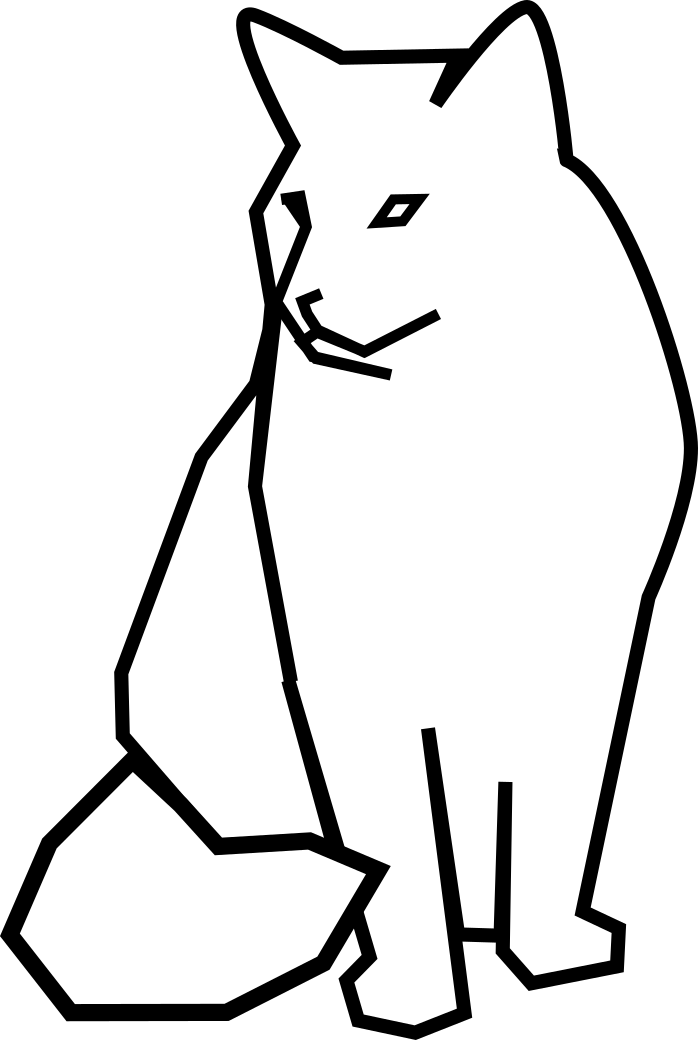
\includegraphics[width=1.8cm]{pictures/betisou.png}\\
        \begin{center}
            "Is this a cat ?"
        \end{center}
    \end{columns}
    \pause

    {\Large Examples:}
    \medskip
    \begin{columns}
        \column{.01\textwidth}
        \column{.48\textwidth}
        {\borange{Lossy: Karp--Rabin fingerprints}}
        \column{.48\textwidth}
        {\bblue{Lossless: Lempel--Ziv factorization}}
    \end{columns}
    
\end{frame}

\begin{frame}{Example of lossy sketch: Karp--Rabin fingerprints}
    \begin{framed}
        Definition: $$ \varphi(P) = P[1]r^{m-1}+P[2]r^{m-2} + \dots + P[m-1]r + P[m] \mod p$$ 
        for $p$ a prime and $r < p$. \pause
        
        Testing if $\varphi(T[i+1..i+m])=\varphi(P)$ can be tested in $\Oh(1)$ and if so the strings match w.h.p.
        \begin{tabular}{l c}
        \textcolor{black}{Sliding window:} & \hspace{1cm}
\includegraphics[width=0.5\textwidth]{pictures/slidding_window.png}
        \end{tabular}
        $$ \varphi(T[i+1..i+m]) = \varphi(T[i..i+m-1])\times r - S[i]r^k + S[i+m] \mod p$$\vspace{-0.5cm}
    \end{framed}
\end{frame}

\begin{frame}{Example of lossless sketch: Lempel--Ziv factorization}
\end{frame}

\begin{frame}{What is a sketch ?}
    \begin{columns}
        \column{.6\textwidth}
        A \textbf{sketch} is a \bblue{lossless} or \borange{lossy} compression that \textbf{keeps only the essential characteristic of the input} needed to answer a specified type of query.\\
        \column{.35\textwidth}
        
\includegraphics[width=1.8cm]{pictures/photo_betisou.jpg}
        \hspace{0.5cm}
        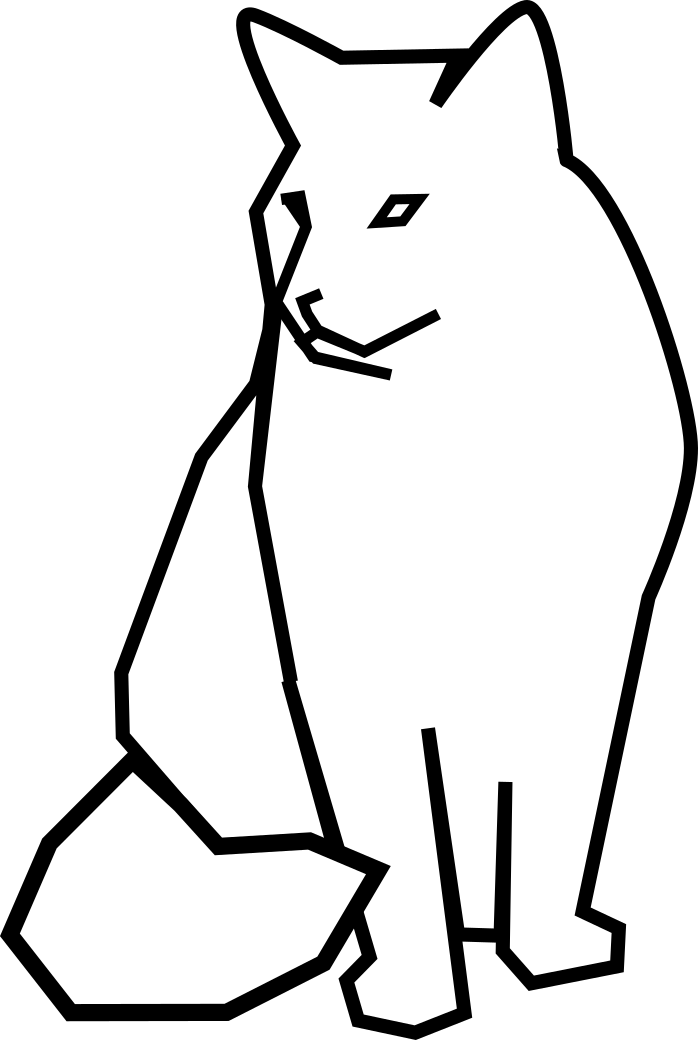
\includegraphics[width=1.8cm]{pictures/betisou.png}\\
        \begin{center}
            "Is this a cat ?"
        \end{center}
    \end{columns}

    {\Large Examples:}
    \medskip
    \begin{columns}
        \column{.01\textwidth}
        \column{.48\textwidth}
        {\borange{Lossy: Karp--Rabin fingerprints}}
        \begin{itemize}
            \item They occupy constant space,  
            \item can check whether two strings match with high probability,
            \item but cannot be used to reconstruct the original string. 
        \end{itemize}
        \column{.48\textwidth}
        {\bblue{Lossless: Lempel--Ziv factorization}}
        \begin{itemize}
            \item It is a very efficient compression in practice (used in \texttt{.png} or \texttt{.zip}),
            \item can reconstruct the original string,
            \item but in the worst case it does not compress. 
        \end{itemize}
    \end{columns}
    
\end{frame}

\begin{frame}{Why should I use sketches and how ?}
    \begin{columns}
        \column{.52\textwidth}
        A \textbf{sketch} is a \bblue{lossless} or \borange{lossy} compression that \textbf{keeps only the essential characteristic of the input} needed to answer a specified type of query.
        \column{0.05\textwidth}
        \LARGE{$\rightarrow$}
        \column{0.33\textwidth}
            Sketches are typically much \bgreen{smaller}, thus can allow \bgreen{scaling to larger} datasets.
    \end{columns}
    \bigskip
    \pause


    \hspace{-0.5cm} {\large \textcolor{black!30!blue}{Three main approaches in this thesis:}}
    \begin{columns}
        \column{0.33\textwidth}
        \begin{framed}
            \begin{center}
                \textbf{Sketch as input}
            \end{center}
            Operating directly on the sketch given as input (not decompressing).
        \end{framed}
        \column{0.66\textwidth}
        \begin{framed}
            \begin{center}
                \textbf{Sketch as you go}
            \end{center}
            Compute the sketch of the input on the fly and use it later on in your algorithm. 
            \begin{itemize}
                \item For Streaming
                \item For approximation
            \end{itemize}
        \end{framed}
    \end{columns}
\end{frame}
